\section{Анализ работы клеточного автомата}

Рассмотрим, как автомат меняет несколько начальных конфигураций.

\subsection{Диагональный паттерн}

Начальное состояние с живыми клетками на диагонали показано на
рисунке~\ref{fig:1-1}. Из-за тороидальных граничных условий диагональ
переходит через край поля (рисунки~\ref{fig:1-2} и~\ref{fig:1-3}). Через
некоторое время конфигурация повторяется; все состояния приведены на
рисунке~\ref{fig:diagonal-pattern}.

\begin{figure}[htbp]
    \centering
    \begin{subfigure}{0.31\linewidth}
        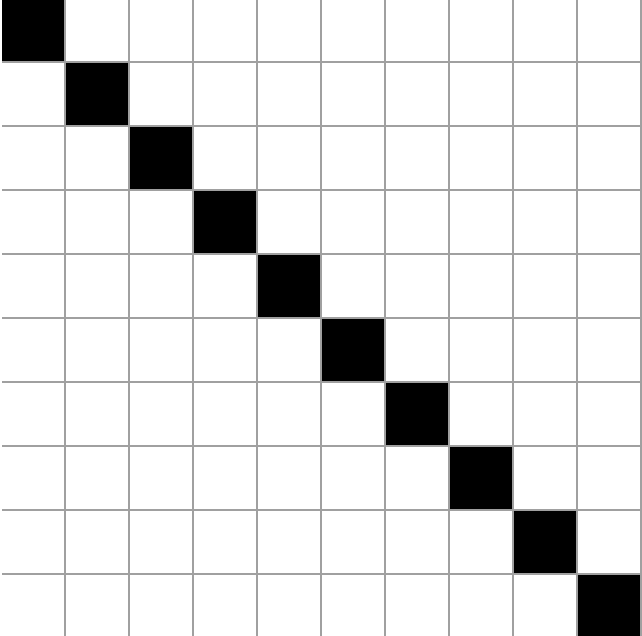
\includegraphics[width=\linewidth]{myPhoto/1-1.png}
        \caption{Начальное состояние}
        \label{fig:1-1}
    \end{subfigure}\hfill
    \begin{subfigure}{0.31\linewidth}
        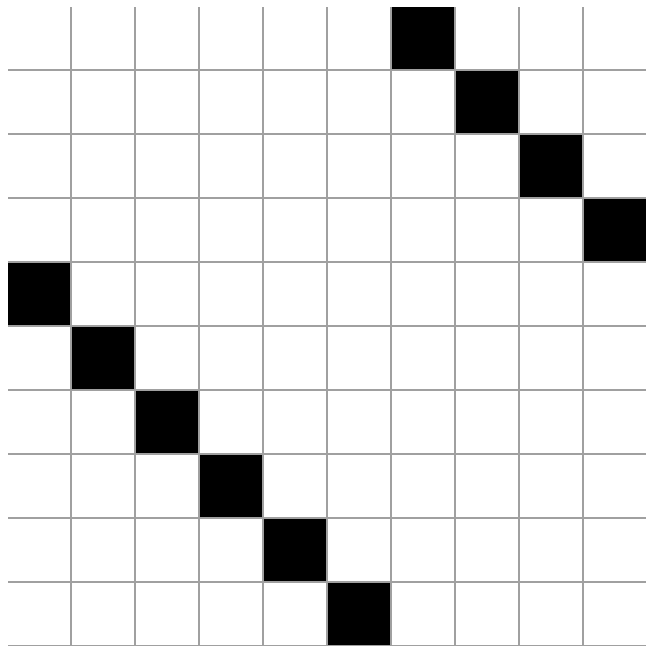
\includegraphics[width=\linewidth]{myPhoto/1-2.png}
        \caption{После четырёх шагов}
        \label{fig:1-2}
    \end{subfigure}\hfill
    \begin{subfigure}{0.31\linewidth}
        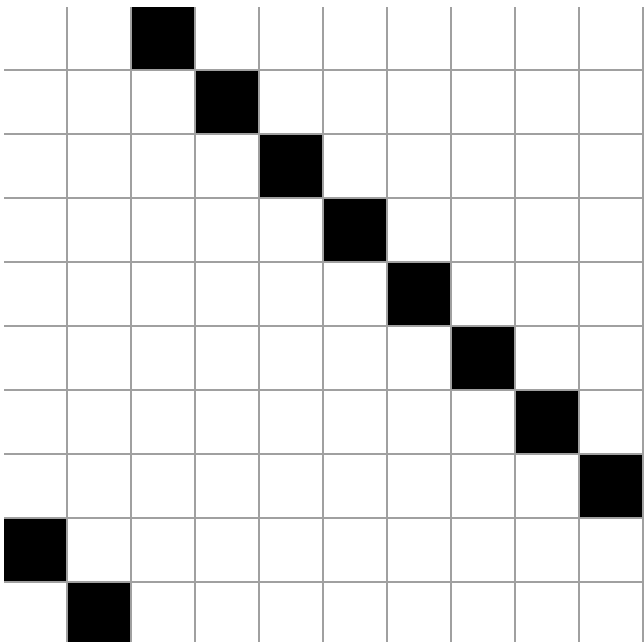
\includegraphics[width=\linewidth]{myPhoto/1-3.png}
        \caption{После дальнейших шагов}
        \label{fig:1-3}
    \end{subfigure}
    \caption{Изменение диагонального паттерна}
    \label{fig:diagonal-pattern}
\end{figure}

\subsection{Шахматный паттерн}

На рисунках~\ref{fig:2-1} и~\ref{fig:2-2} показаны два состояния
шахматного паттерна. На каждом шаге живые и мёртвые клетки меняются
местами, поэтому эти состояния чередуются с периодом два шага.

\begin{figure}[htbp]
    \centering
    \begin{subfigure}{0.44\linewidth}
        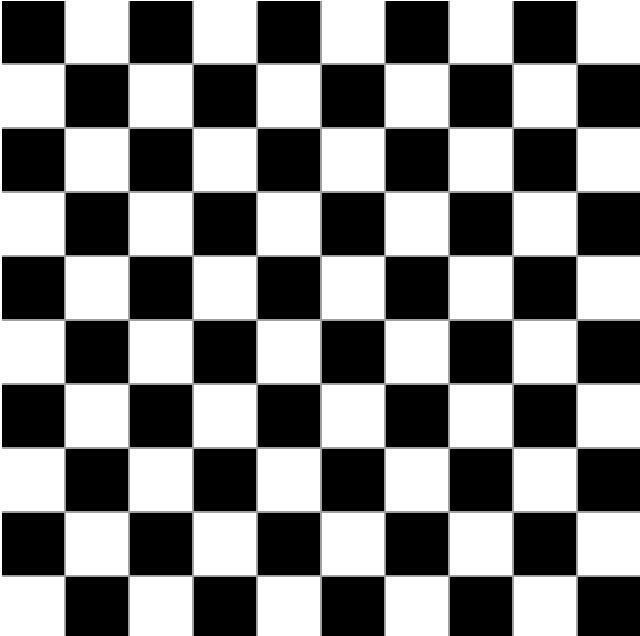
\includegraphics[width=\linewidth]{myPhoto/2-1.png}
        \caption{Первое состояние}
        \label{fig:2-1}
    \end{subfigure}\hfill
    \begin{subfigure}{0.44\linewidth}
        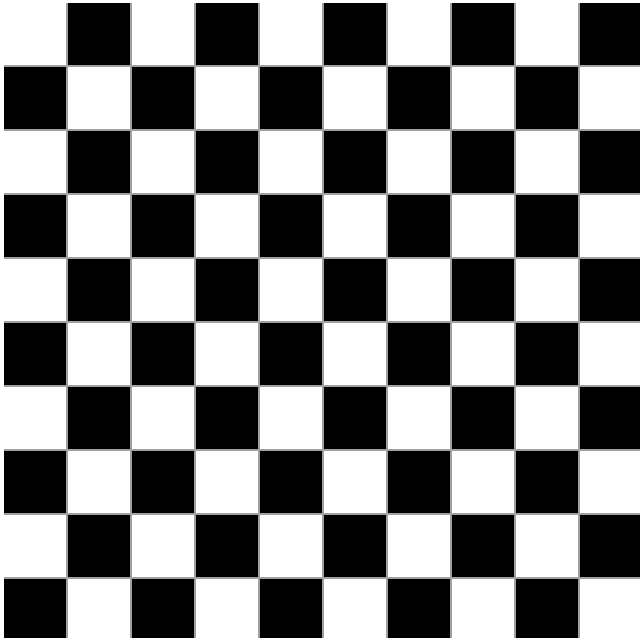
\includegraphics[width=\linewidth]{myPhoto/2-2.png}
        \caption{После одного шага}
        \label{fig:2-2}
    \end{subfigure}
    \caption{Чередование состояний шахматного паттерна}
    \label{fig:checkerboard-pattern}
\end{figure}

\subsection{Случайное заполнение поля}

При случайном заполнении поля начальное состояние (рисунок~\ref{fig:3-1})
постепенно упрощается. На рисунке~\ref{fig:3-2} видны оставшиеся
вертикальные пары живых клеток; увеличенная пара показана на
рисунке~\ref{fig:random-pair}.

Пара сохраняется из-за правила перехода:
$f(1,0,1,0,0)=1$ для верхней клетки и $f(1,1,0,0,0)=1$ для нижней.
Соседние мёртвые клетки не загораются: для их наборов правило возвращает
0. Поэтому пара не исчезает и не разрастается.

\begin{figure}[htbp]
    \centering
    \begin{subfigure}{0.44\linewidth}
        
\includegraphics[width=\linewidth]{myPhoto/3-1.png}
        \caption{Начальное случайное состояние}
        \label{fig:3-1}
    \end{subfigure}\hfill
    \begin{subfigure}{0.44\linewidth}
        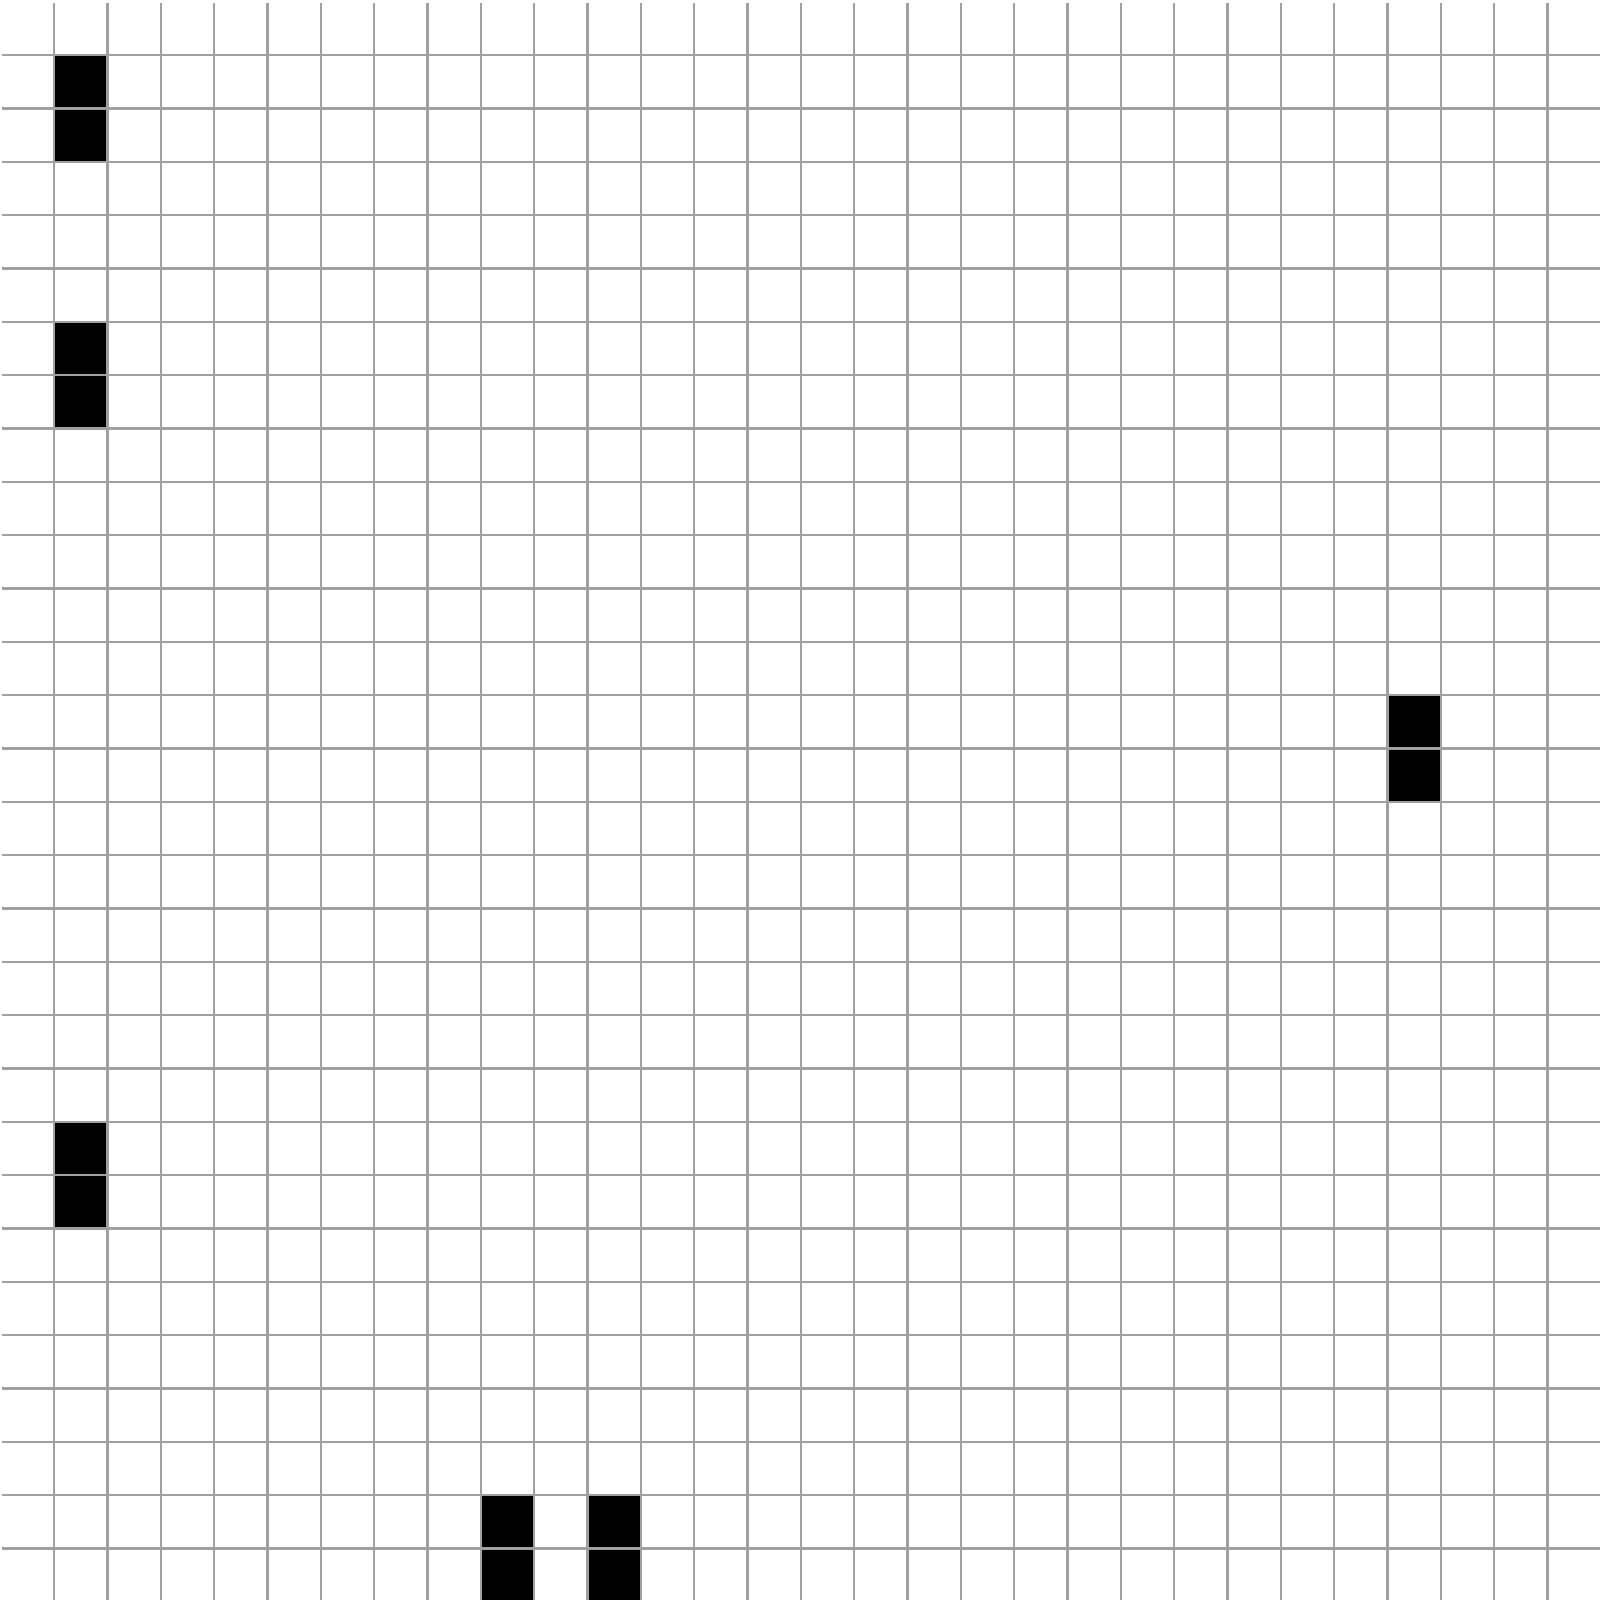
\includegraphics[width=\linewidth]{myPhoto/3-2.png}
        \caption{После нескольких шагов}
        \label{fig:3-2}
    \end{subfigure}
    \caption{Изменение случайной конфигурации}
    \label{fig:random-pattern}
\end{figure}

\begin{figure}[htbp]
    \centering
    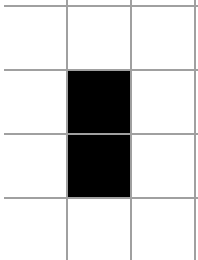
\includegraphics[width=0.16\linewidth]{myPhoto/3-3.png}
    \caption{Увеличенный фрагмент с устойчивой парой клеток}
    \label{fig:random-pair}
\end{figure}

\subsection{Крестообразный паттерн}

Начальное состояние крестообразного паттерна показано на рисунке~\ref{fig:4-1}.
После нескольких шагов клетки располагаются иначе (рисунок~\ref{fig:4-2}),
а затем конфигурация становится периодической. Оба состояния показаны на
рисунке~\ref{fig:cross-pattern}.

\begin{figure}[htbp]
    \centering
    \begin{subfigure}{0.44\linewidth}
        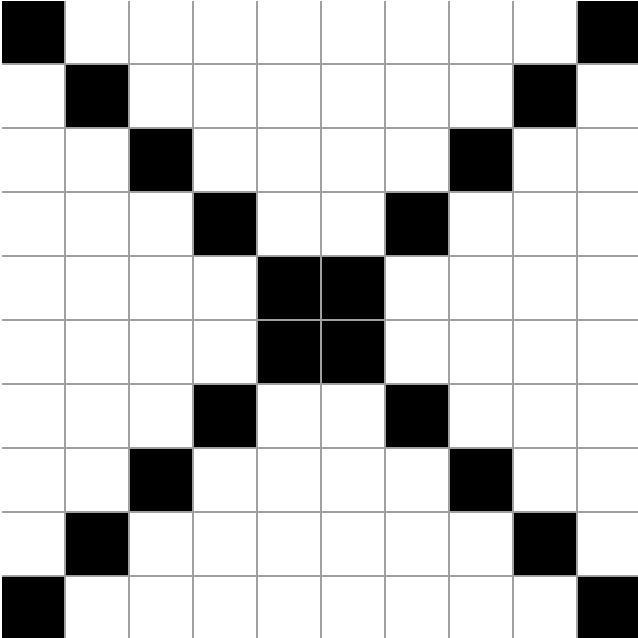
\includegraphics[width=\linewidth]{myPhoto/4-1.png}
        \caption{Начальное состояние}
        \label{fig:4-1}
    \end{subfigure}\hfill
    \begin{subfigure}{0.44\linewidth}
        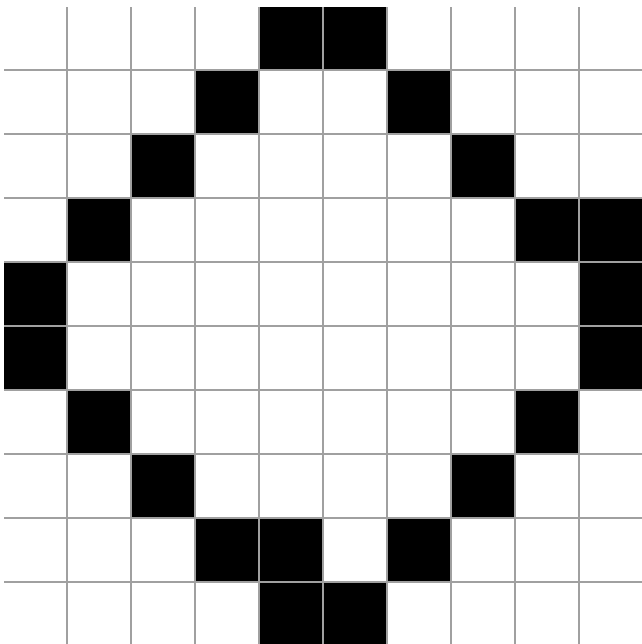
\includegraphics[width=\linewidth]{myPhoto/4-2.png}
        \caption{После нескольких шагов}
        \label{fig:4-2}
    \end{subfigure}
    \caption{Изменение крестообразного паттерна}
    \label{fig:cross-pattern}
\end{figure}

\subsection{Класс автомата по Вольфраму}

По рассмотренным примерам автомат ближе ко II классу: случайное поле
упрощается до устойчивых пар, а другие паттерны повторяются через несколько
шагов. Признаков хаотичного поведения III и IV классов в этих опытах нет.

\subsection{Сходимость и количество клеток}

Для численного анализа поле размером $30\times30$ было заполнено случайными
значениями. Для повторяемости эксперимента использовалось одинаковое
начальное значение генератора случайных чисел (seed).
На каждом шаге подсчитывались живые клетки $B_t$ и мёртвые клетки $W_t$;
всегда выполняется $B_t+W_t=900$. Сходимость оценивалась по доле живых
клеток $\rho_t=B_t/900$. Постоянная доля означает, что число живых клеток
не меняется, но поле при этом ещё может изменяться. Поэтому дополнительно
сравнивались конфигурации соседних шагов.

В начале было 440 живых клеток ($\rho_0\approx0{,}489$), к шагу 15 осталось
18 ($\rho_{15}=0{,}02$). Доля не менялась до шага 200. Состояния поля на
шагах 15 и 16 также совпали, поэтому в этом запуске поле стало неподвижным.

\begin{center}
    \captionof{table}{Количество и доля живых клеток}
    \label{tab:random-field-metrics}
    \begin{tabular}{|c|r|c|}
        \hline
        Шаг $t$ & Живые $B_t$ & Доля $\rho_t$ \\
        \hline
        0   & 440 & 0{,}489 \\
        5   & 70  & 0{,}078 \\
        10  & 25  & 0{,}028 \\
        15  & 18  & 0{,}020 \\
        200 & 18  & 0{,}020 \\
        \hline
    \end{tabular}
\end{center}

На рисунке~\ref{fig:random-30-metrics} показано изменение доли живых клеток.
Полный набор значений за 200 шагов приведён в приложении Б.

\begin{center}
    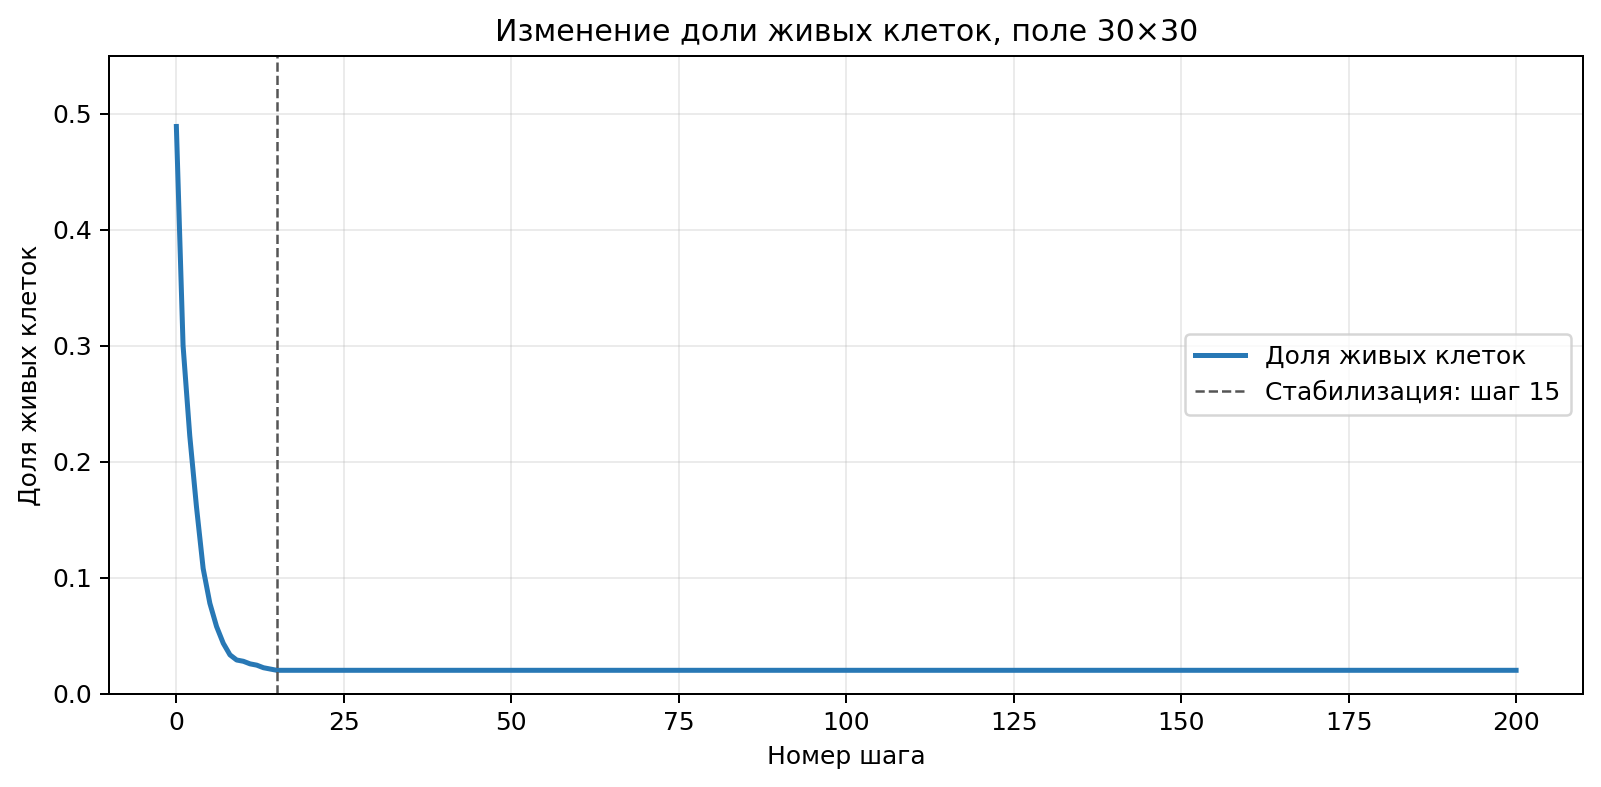
\includegraphics[width=0.85\linewidth]{myPhoto/random_30x30_metrics.png}
    \captionof{figure}{Доля живых клеток в случайном поле 30$\times$30}
    \label{fig:random-30-metrics}
\end{center}
